
%%%%%%%%%%%%%%%%%%%%%%
% Next year, design an active low-pass filter, which is basically the same circuit as an integrator but connect a resistor in parallel with a capacitor. 
%%%%%%%%%%%%%%%%%%%%%%

\section{Objectives}
By the end of this laboratory experiment, students are expected to learn how to 

\begin{itemize}

\item work with operational amplifiers and   
  
\item build integrator and square wave voltage tracking circuits using inverting operational amplifiers.  
 
  
\end{itemize}

\section{Parts}
\label{sec:partsEx9}
The following parts are required to conduct this laboratory experiment. %
%
\begin{enumerate}
\item Breadboard
\item One single-pole, single-throw (SPST) switch
\item Three LMC6482\footnote{See its datasheet at \href{http://www.ti.com/lit/ds/symlink/lmc6482.pdf}{http://www.ti.com/lit/ds/symlink/lmc6482.pdf}} dual operational amplifier ICs
  
% \item Three LF412\footnote{See its datasheet at \href{http://www.ti.com/lit/ds/snosbh7f/snosbh7f.pdf}{http://www.ti.com/lit/ds/snosbh7f/snosbh7f.pdf}} dual operational amplifier ICs\footnote{LM741 operational amplifier ICs will be used in case LF412 ICs are not available}, 
\item Nine $10~[\kilo\ohm]$ resistors, and     
\item Two $0.1~[\micro\farad]$ capacitors.  
\end{enumerate}

\section{Background}
\label{sec:background}

This experiment deals with applications of operational amplifiers, which are active electronic devices. An operational amplifier consists of transistors, resistors, diodes, and capacitors, all fabricated and inter-connected into a single tiny chip (also called an integrated circuit (IC)). It is typically a five terminal device as shown in Figure~\ref{fig:opAmp}.  The ``+'' and the ``-'' symbols indicate the non-inverting and inverting input terminals, respectively. The time-varying input signals, $v_{i_1}(t)$ and $v_{i_2}(t),$ for time $t\ge 0,$ are applied at the input terminals of the operational amplifier. Note that the ``+'' and the ``-'' symbols are not to be confused with the polarity of the input signals, $v_{i_1}(t)$ and $v_{i_2}(t).$ The output of the operational amplifier is taken from the output terminal labeled $v_o(t).$   The positive and negative power supply voltages are labeled as $V_{\text{CC}}$ and $-V_{\text{EE}}$ (or $V^+$ or $V^-),$ respectively, which are required for an operational amplifier to operate as an active electronic device. The circuit symbol for an operational amplifier is given in Figure~\ref{fig:opAmpSymbol}, where power supply voltages are not shown. %
%
\begin{figure}
  \centering
  \subfigure[][]{
    \label{fig:opAmp}
  \begin{circuitikz}[scale=1.2,american voltages]
    \draw % 
    (0,0) node[op amp,fill=cyan!50] (opAmp) {};
    \draw 
    (opAmp.-) node[left]{Inverting input, $v_{i_1}(t)$}
    (opAmp.+) node[left]{Non-inverting input, $v_{i_2}(t)$}
    (opAmp.out) node[right]{Output, $v_o(t)$};
    \draw 
    (opAmp.up) --++(0,0.7) node[vcc]{Positive power supply, $+V_{\text{CC}}=V^{+}$}  % ++(0,0.7) means have the node lable Vcc 0.7 up from the previous default Vcc label
    (opAmp.down)--++(0,-0.7) node[vee]{Negative power supply, $-V_{\text{EE}}=V^{-}$};  % ++(0,-0.7) means have the node lable Vee 0.7 down from the previous default Vee label     
  \end{circuitikz}
}
\subfigure[][]{
  \label{fig:opAmpSymbol}
  \begin{circuitikz}[scale=5,american voltages]
    \draw % 
    (0,0) node[op amp,fill=cyan!50] (opAmp) {}
    (opAmp.-) node[left]{$v_{i_1}(t)$}
    (opAmp.+) node[left]{$v_{i_2}(t)$}
    (opAmp.out) node[right]{$v_o(t)$};
  \end{circuitikz}
}
  \caption{\subref{fig:opAmp} An operational amplifier and its \subref{fig:opAmpSymbol} circuit symbol.}
  \label{fig:operationalAmplifier}
\end{figure}
%
Since we will be dealing with the frequency response of a circuit using operational amplifiers, it is important to discuss some definitions associated with the Laplace tranformation of a time-domain function $y(t).$

  \begin{definition}[Complex variable]
    A complex number (complex frequency) has a real part and an imaginary part, both
    of which are constant.
    $$s = \sigma + j\omega$$
    where $\sigma$ is the real part and $\omega$ is the imaginary part. 
  \end{definition}
  \begin{definition}[Complex function]
A complex function $G(s)$, a function of $s$, has a real part and an imaginary part, or: 
$$G(s) = G_x + jG_y,$$
where $G_x$ and $G_y$ are real quantities. The magnitude of $G(s)$ is $\sqrt{G_x^2+G_y^2},$ and the angle $\theta$ of $G(s)$ is $\tan^{-1}(G_y/G_x)$. The angle is measured counterclockwise from the positive real axis. The complex conjugate of $G(s)$ is $G^*(s) = G_x-jG_y.$ 
\end{definition}

\begin{definition}[Laplace transformation (LT)]
  The Laplace transformation of a time-domain function $y(t),$ for time $t\ge 0$ is given by %  
  \begin{equation*}
\mathscr{L}\left[y(t)\right]  = Y(s) =\int_0^\infty \left[y(t)\right]e^{-st} \mathrm{dt},~~\text{where}
  \end{equation*}
\begin{tabular}{lll}
$y(t)$   & $\equiv$ & function of time $t$ such that $y(t)=0$ for $t<0,$\\
$s$&$\equiv$&a complex variable,\\
$\mathscr{L}$&$\equiv$& Laplace transformation operator, and \\
$Y(s)$&$\equiv$&Laplace transform of $y(t).$
\end{tabular}    
  \end{definition}
  \begin{definition}[Inverse Laplace transform]
    The inverse Laplace transformation determines the time domain function $y(t)$ given $Y(s).$ This is described by % 
    \begin{equation*}
      \mathscr{L}^{-1}\left[Y(s)\right]  = y(t) =  \frac{1}{2\pi j}\int_{\sigma -j\omega}^{\sigma +j\omega} Y(s)e^{st} \mathrm{ds},~~\text{for}~t > 0.
    \end{equation*}
%where $c$,the abscissa of convergence, is a real constant and is chosen larger than the real parts of all singular points of $F(s)$.
  \end{definition}

  \subsection{Transfer Function (TF) and Bode Plots}
\label{sec:transferFunction}
Linear two-port electrical circuits are modeled by transfer functions (TFs). Transfer function (\textit{i.e.,} Laplace TF) models are based on Laplace transformations. An electrical circuit (or system) with one input and one output can be uniquely represented by a TF.   Assume $V_i(s)$ and $V_o(s)$ are Laplace transforms of an input signal $v_i(t)$ and an output signal $v_o(t)$ for time $t\ge 0,$ (respectively) of an electrical circuit. The Laplace TF is then defined as %
  %
  \begin{align}
    G(s) = \frac{\text{LT of output}}{\text{LT of input}}=\frac{V_o(s)}{V_i(s)}.
    \label{eq:LaplaceTF}
  \end{align}
  %
Substituting $s=j\omega = j2\pi f$ yields the frequency TF (also called the \emph{frequency response}), which is given by %
\begin{align}
    H(f) = \frac{V_o(f)}{V_i(f)},
\end{align}
where $f$ is the frequency (in~[\hertz]) of the input signal. The frequency TF $H(f)$ is characterized by Bode plots, which are a pair of plots: one showing the magnitude of $H(f)$ in [\decibel] versus frequency in logarithmic scale  and the other one showing the angle of $H(f)$ in [degree (\degree)] versus frequency in logarithmic scale. 

\subsection{Impedance of Passive Linear Electrical Components}
\label{sec:TF-Passive}
The electrical circuits that are used throughout this laboratory consists of three passive linear components: resistors, capacitors, and inductors. Let $R,$ $C,$ and $L$ denote the resistance, capacitance, and inductance. Assume $V_R(s)$ and $I_R(s)$ denote  the Laplace transforms of the voltage across and the current flowing through a resistor. The impedance (in Laplace domain) of a resistor, $Z_R(s),$ is  given by %
%
\begin{align*}
  Z_R(s) &= \frac{V_R(s)}{I_R(s)}  = R.
  % Z_R(s) &= \frac{V_R(s)}{I_R(s)}  = R\\  
\end{align*}
%
Similarly, the impedances of a capacitor, $Z_C,$ and an inductor, $Z_L,$ are given by: %
%
\begin{align*}
  Z_C(s) &= \frac{V_C(s)}{I_C(s)}  = \frac{1}{Cs},~\text{and}\\
  Z_L(s) &= \frac{V_L(s)}{I_L(s)}  = Ls,\\  
\end{align*}
%
respectively, where $V_C(s)$ and $I_C(s)$ are Laplace transforms of the voltage across and the current flowing through a capacitor, and $V_L(s)$ and $I_L(s)$ are Laplace transforms of the  voltage across and the current flowing through an inductor, respectively. 

  
\section{Integrator}
\label{sec:integrator}
%
This section illustrates a simple integrator circuit using an inverting operational amplifier. The input to the integrator  is a sinusoidal voltage signal given by $v_i(t) = A\sin(\omega t), $ with $A$ being the maximum amplitude, $\omega=2\pi f$ is the angular frequency in $[\si{\radian\per\second}]$, and $f$ is the frequency in $[\hertz].$ The desired  output voltage is $v_o(t) = K_I\int_0^tv_i(t)\mathrm{dt}$ for some $K_I>0.$  The block diagram for this simple integrator system is given in Figure~\ref{fig:integratorBlockDiagram}. The circuit diagram of  the integrator is shown in Figure~\ref{fig:integrator}, where $R$ is the resistance and $C$ is the capacitance. The reset switch (when closed) has the effect of resetting the integrator to zero by discharging the capacitor.  
%
\begin{figure}
  \centering
  \begin{circuitikz}
    \draw [fill=lightgray]
    (0,0) rectangle (5*\smgrid,3*\smgrid);
    \node at (2.5*\smgrid,1.5*\smgrid) {Integrator};
    % Input 
    \draw[-latex]
    (-\smgrid,1.5*\smgrid) node[left]{$v_i(t)=A\sin(\omega t)$} -- (0*\smgrid,1.5*\smgrid);
    \draw[-latex] % Output
    (5*\smgrid,1.5*\smgrid) -- (6*\smgrid,1.5*\smgrid) node[right]{$v_o(t)=K_I\int_0^tv_i(t)\mathrm{dt}$};    
  \end{circuitikz}
  \caption{Block diagram of an integrator system. }
  \label{fig:integratorBlockDiagram}
\end{figure}
%
\begin{figure}
  \centering
  \begin{circuitikz}[american voltages]
    % \tikzstyle{every node} = [font=\tiny]
    \draw 
    (8.0*\smgrid,-0.5)node[op amp,fill=cyan!50](opampIntegrator){};
    \draw
    (0,0) to[R,l^=$R$, o-*] (4*\smgrid,0) --(opampIntegrator.-);
    \draw
    (4*\smgrid,0) |- (4*\smgrid,3*\smgrid) to[C,l=$C$] (10*\smgrid,3*\smgrid) -|(opampIntegrator.out) to[short,*-o] (11*\smgrid,-0.5);%node[right]{$v_o(t)$};
    \draw
    (4*\smgrid,3*\smgrid) --  (4*\smgrid,6*\smgrid) to[opening switch, l= Reset switch$\Rightarrow t{=}0~{[}\second{]}$] (10.37*\smgrid,6*\smgrid) --(10.37*\smgrid,3*\smgrid);
    \draw
    (0,-1.0)node[ground]{} to[short,o-] (opampIntegrator.+);
    \draw
    (-0.2,-.8) to[open,v<=$v_i(t)$] (-0.2,0);
    \draw
    (11*\smgrid,-1.0) to[short,-o] (11*\smgrid,-1.0)node[ground]{};
    \draw
    (11.4*\smgrid,-0.8) to[open,v<=$v_o(t)$] (11.4*\smgrid,-0.7);
  \end{circuitikz}
  \caption{An integrator circuit using an inverting operational amplifier.}
  \label{fig:integrator}
\end{figure}
%
Clearly, the Laplace transforms of the impedances of the resistance and the capacitance are $Z_R(s) = R$ and $Z_C=\frac{1}{Cs}.$ If the Laplace transforms of the input and output voltages are $V_i(s)$ and $V_o(s),$ respectively, then  the transfer function of the integrator is given by %
%
\begin{align}
  G(s) = \frac{V_o(s)}{V_i(s)} = -\frac{Z_C(s)}{Z_R(s)} = -\frac{1}{RCs}
  \label{eq:TF-Integrator}
\end{align}
%
Substituting $s=j\omega=2\pi f$ in Equation~\eqref{eq:TF-Integrator}, we get the frequency response (\textit{i.e.,} frequency TF) of the integrator, $H(f),$ given by %
%
\begin{align}
  H(f) = -\frac{1}{j2\pi fRC},
  \label{eq:frequencyTF-Integrator}
\end{align}
%
where $f$ is the frequency of the input voltage $v_i(t).$The output of the integrator circuit is given by: %
%
    \begin{equation}
      v_o(t)= \mathscr{L}^{-1}\left[V_o(s)\right]  = \mathscr{L}^{-1}\left[G(s)V_i(s)\right]  = \frac{A}{2\pi fRC}\cos(\omega t),
      \label{eq:integratorOutput}
    \end{equation}
%

    for $t\ge 0.$

\section{Tracking Square Wave Signal }
\label{sec:followingSquareWave}

In this part, we will be using the second-order circuit shown in~\autoref{fig:secondOrderCircuitOpAmp}, where $x_2(t)$ is the output of \emph{op-amp~\#1} of the circuit. %
%
\begin{figure}
  \centering
  \begin{circuitikz}[scale=1,american voltages]
    \draw
    (0,0) node[op amp,fill=cyan!50] (opamp1){}
    (-8*\smgrid,\smgrid) node[left]{$v_i(t)$} to[R,l^=$R_1$,o-*](opamp1.-)
    (opamp1.+)to[short,-*](opamp1.+)node[ground]{};
    \node at(0,0){\#1};
    \draw
    (opamp1.-) to[short,-](-2.4*\smgrid,4*\smgrid) to[C,l^=$C_1$](2.4*\smgrid,4*\smgrid) to[short,-*](opamp1.out);
    
    \draw
    (10*\smgrid,-\smgrid) node[op amp,fill=cyan!50](opamp2){}
    (opamp1.out)node[below]{$x_2(t)$} to[R,l^=$R_2$,-*](opamp2.-)
    (opamp2.-) to[short,-](7.5*\smgrid,4*\smgrid) to[C,l^=$C_2$](12.4*\smgrid,4*\smgrid) to[short,-*](opamp2.out);
    \node at(10*\smgrid,-\smgrid){\#2};
    \draw 
    (opamp2.+) to[short,-*](opamp2.+)node[ground]{};
    
    \draw 
    (opamp2.-) |-(5*\smgrid,-\smgrid) to[short,-] (5*\smgrid,-6*\smgrid) to[R,l_=$R_3$](12.3*\smgrid,-6*\smgrid) -- (opamp2.out);

    \draw
    (opamp2.out) to[short,-o](14*\smgrid,-\smgrid) node[right]{$v_o(t)$};
    
  \end{circuitikz}
  \caption{A second-order circuit using inverting operational amplifiers.}
  \label{fig:secondOrderCircuitOpAmp}
\end{figure}
%
The corresponding block diagram of the second order circuit is shown in~\autoref{fig:secondOrderCircuitOpAmpBD}, where $G_1(s)$ and $G_2(s)$ are the transfer functions of the \emph{Op-amp \#1} and \emph{Op-amp \#2} circuits, respectively. 
%
\begin{figure}
  \centering
  \begin{circuitikz}
    \draw [fill=lightgray]
    (0,0) rectangle (5*\smgrid,3*\smgrid);
    \node at (2.5*\smgrid,1.5*\smgrid) {$G_1(s)$};
    % Input 
    \draw[-latex]
    (-\smgrid,1.5*\smgrid) node[left]{$V_i(s)$} -- (0*\smgrid,1.5*\smgrid);
    \draw % Output
    (5*\smgrid,1.5*\smgrid) -- (7*\smgrid,1.5*\smgrid) node[below]{$X_2(s)$};

    \draw [fill=lightgray]
    (10*\smgrid,0) rectangle (15*\smgrid,3*\smgrid);
    \node at (12.5*\smgrid,1.5*\smgrid) {$G_2(s)$};
    % Input 
    \draw[-latex]
    (7*\smgrid,1.5*\smgrid) -- (10*\smgrid,1.5*\smgrid);
    \draw[-latex] % Output
    (15*\smgrid,1.5*\smgrid) -- (17*\smgrid,1.5*\smgrid) node[right]{$V_o(s)$};    
  \end{circuitikz}
  \caption{Equivalent block diagram of the second-order circuit shown in~\autoref{fig:secondOrderCircuitOpAmp}. }
  \label{fig:secondOrderCircuitOpAmpBD}
\end{figure}
%
Clearly, %
\begin{align*}
  X_2(s) &= G_1(s)V_i(s) = -\frac{1}{R_1C_1s}V_i(s),\\
  V_o(s) &= G_2(s)X_2(s) = \left(-\frac{\frac{R_3}{1+R_3C_2s}}{R_2}\right)\times 			
           \left(-\frac{1}{R_1C_1s}V_i(s)\right)V_i(s)= \frac{R_3}{R_1C_1R_2C_2R_3s^2+R_1C_1R_2s}V_i(s).  
\end{align*}
%
Therefore, the transfer function of the second-order circuit is given by %
%
\begin{align}
  G_P(s)=\frac{V_o(s)}{V_i(s)} = \frac{R_3}{R_1C_1R_2C_2R_3s^2+R_1C_1R_2s}.
  \label{eq:oltf}
\end{align}
%
Assuming $R_1=R_2=R_3=R$ and $C_1=C_2=C$, Equation~\eqref{eq:oltf} yields:
	\begin{align}
          G_P(s) = \frac{R}{R^3C^2s^2+R^2Cs}= \frac{1}{R^2C^2s^2+RCs} \equiv \frac{\omega_n^2}{s^2+2\zeta\omega_ns}\equiv\frac{1}{\frac{1}{\omega_n^2}s^2+2\times \frac{\zeta}{\omega_n}s}.
          \label{eq:oltf1}
	\end{align}
        %
Equating the co-efficients of Equation~\eqref{eq:oltf1} gives the natural frequency $\omega_n= \frac{1}{RC}$ and the damping ratio $\zeta=0.5.$  Note that the circuit shown in~\autoref{fig:secondOrderCircuitOpAmp} does not produce an output signal $v_o(t)$ that tracks the square wave input signal $v_i(t).$ The proof is omitted for the purpose of conciseness. Therefore, the circuit in~\autoref{fig:secondOrderCircuitOpAmp} needs to be modified. A possible circuit whose output voltage tracks a square wave input voltage is given in~\autoref{fig:pControllerCircuit}. %
%
\begin{figure}[htbp]
  \centering
  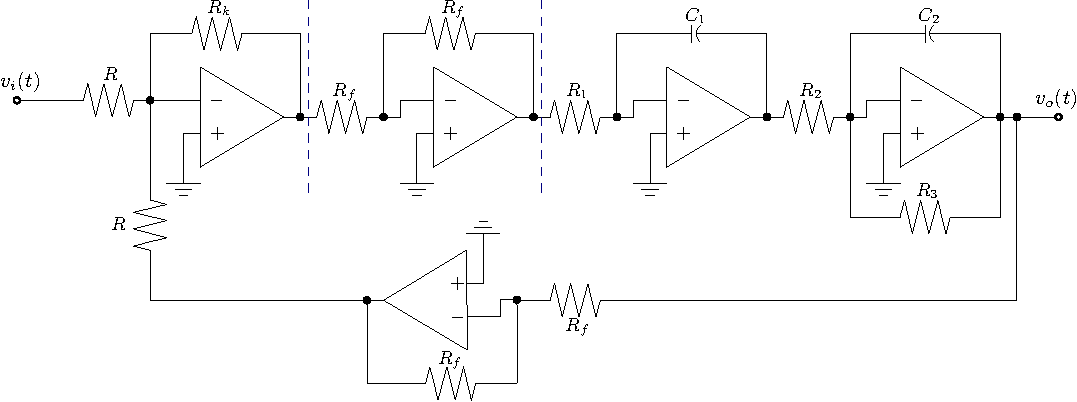
\includegraphics[width=0.8\textwidth]{figs/ipe/lab8/pControllerCircuit}
  \caption[]{Voltage follower circuit using Op-Amp.}
  \label{fig:pControllerCircuit}
\end{figure}
%


The closed--loop transfer function of the circuit shown in~\autoref{fig:pControllerCircuit} is given by %         
%
\begin{align}
  \boxed{
  G_{\text{cl}}(s) = \frac{V_o(s)}{V_i(s)}=\frac{\frac{K_P\omega_n^2}{s^2+2\zeta\omega_ns}}{1+\frac{K_P\omega_n^2}{s^2+2\zeta\omega_ns}}=\frac{K_P\omega_n^2}{s^2+2\zeta\omega_ns+K_P\omega_n^2}.}
  % \label{eq:cltf-pcontroller}  
\end{align}
%
The value of $K_P$ can be found from the ratio of resistances $R_k$ and $R,$ \textit{i.e.,}~$K_P=\frac{R_k}{R}.$

%%%%%%% Figure 2.11  of Nise (PID controller circuit)

% \begin{figure}
%   \centering
%   \begin{circuitikz}[scale=1,american voltages]
%     \draw
%     (0,0) to[short,-o](0,0) node[left]{$v_i(t)$} -| (\smgrid,2*\smgrid) to[C,l^=$C_1$](5*\smgrid,2*\smgrid) --(5*\smgrid,-2*\smgrid) to[R,l^=$R_1$](\smgrid,-2*\smgrid) -- (\smgrid,0);
%     \draw
%     (12*\smgrid,-\smgrid) node[op amp](opamp3){};
%     \draw
%     (7*\smgrid,0*\smgrid) -- (opamp3.-)node[anchor=south]{$v_1(t)$};
%     \draw
%     (opamp3.+) to[short,-*](opamp3.+) node[ground]{};
%     \draw
%     (5*\smgrid,0) -| (7*\smgrid,2*\smgrid) to [R,l^=$R_2$] (11*\smgrid,2*\smgrid) to[C,l^=$C_2$](14.4*\smgrid,2*\smgrid) to[short,-*](opamp3.out) to[short,-o](16*\smgrid,-\smgrid)node[right]{$v_o(t)$};    
    
    
%   \end{circuitikz}
%   \caption{Time-varying voltage tracker circuit using inverting operational amplifier.}
%   \label{fig:secondOrderCircuitVoltageTracker}
% \end{figure}



% \section{Noninterting Operational Amplifier}  % Figure 2.13 of Nise 
% \label{sec:non-invertingOpAmp}

% \begin{figure}
%   \centering
%   \begin{circuitikz}[scale=1,american voltages]
%     \draw
%     (5*\smgrid,\smgrid) node[op amp](opamp4){};
%     \draw 
%     (0,0) to[short,-o](0,0) node[left]{$v_i(t)$} --(opamp4.+);

%     \draw
%     (opamp4.out) to[short,*-] (7.4*\smgrid,7*\smgrid) to[C,l_=$C_2$](1.5*\smgrid,7*\smgrid) to[short,-](1.5*\smgrid,-\smgrid) to [R,l_=$R_1$](1.5*\smgrid,-4*\smgrid) to[C,l_=$C_1$] (1.5*\smgrid,-8*\smgrid)node[ground]{};
%     \draw
%     (1.5*\smgrid,2*\smgrid) to[short,*-](opamp4.-) node[anchor=south]{$v_1(t)$};
%     \draw
%     (1.5*\smgrid,4*\smgrid) to[R,*-*,l^=$R_2$](7.4*\smgrid,4*\smgrid);
%     \draw
%     (opamp4.out) to[short,-o](9.4*\smgrid,\smgrid)node[right]{$v_o(t)$};    
    
%   \end{circuitikz}
%   \caption{Non-Inverting operational amplifier circuit.}
%   \label{fig:non-invertingOpamp}
% \end{figure}

\section{Prelab}
\label{sec:prelab}

The prelab of this experiment  consists of three parts. In the first part, you are to analyze the integrator circuit shown in \autoref{fig:integrator}. This is followed by analyzing a second-order op-amp circuit shown in Figure~\ref{fig:secondOrderCircuitOpAmp} in the second part. In the third part, you will be using the second-order circuit in Figure~\ref{fig:secondOrderCircuitOpAmp} to analyze a voltage tracking circuit which is  shown in Figure~\ref{fig:pControllerCircuit}.

% is mainly focused on rectifier circuits. It consists of three parts. In the first part, you are to discuss the operating principles of the circuit that emulates the flashing red light at an intersection (see Figure~\ref{fig:flashingLED}) and the traffic light controller circuit shown in Figure~\ref{fig:TLC}. In the second part, you will analyze the half-wave rectifier circuit shown in Figure~\ref{fig:halfWaveRectifier}. In the third part, the effect of full-bridge diode rectifier circuits is observed in converting an AC voltage signal into a nearly DC signal. %
%
\begin{prelab}[Op-amp integrator]{prelab:integrator}
Consider the integrator circuit shown in Figure~\ref{fig:integrator} with $R =  10~[\kilo\ohm]$  and $C= 0.1~[\micro\farad].$   

\begin{enumerate}
\item Find the  expression of the transfer function, $G(s) = \frac{V_{\mathrm{o}}(s)}{V_{\mathrm{i}}(s)},$ in the complex frequency (Laplace) domain.
  
\item Find the expression of the frequency transfer function $H(f).$
  
\item Plot Bode magnitude and phase of the frequency transfer function, $H(f),$ versus frequency $f\in[0.1,10^4]~\hertz$ (two separate plots) using MATLAB. 


\item In one plot, show the input, $v_i(t)$ and output $v_o(t)$ if $v_i(t) = A\sin(4000\pi t),$ for $t\in[0, 100T_s]~[\second]$ where  $T_s = (0.1)\times 1/(2f_{\mathrm{max}})$ is the sampling time, and $f_{\mathrm{max}}$ is the maximum frequency in~[\hertz], $A = 5~[\volt],$ $R=10~[\kilo\ohm],$ and $C = 0.1~[\micro\farad].$

\item Determine $v_o(t) = -\frac{1}{RC}\int_0^tv_i(t)\mathrm{dt} = -\frac{1}{RC}\int_0^t A\sin(4000\pi t)\mathrm{dt}$ and check with the output voltage waveform found in the previous step.   
\end{enumerate}
\end{prelab}


\begin{prelab}[Tracking square wave voltage]{prelab:pController}
  
Consider the circuit shown in \autoref{fig:secondOrderCircuitOpAmp} with $R_1=R_2 =R_3 = R = 10~[\kilo\ohm]$  and $C_1= C_2=C=0.1~[\micro\farad].$ %
%
\begin{enumerate}
\item Find the  expression of the transfer function, $G_P(s) = \frac{V_{\mathrm{o}}(s)}{V_{\mathrm{i}}(s)},$ in the complex frequency (Laplace) domain. %
  %
\item Find the  values of $\omega_n$ and $\zeta.$  
\item Using the ``square'' function in Matlab, plot a $10~[\hertz]$ square wave signal of amplitude $4~[\volt]$ peak-to-peak for time $t\in[0,0.2]~[\second].$ [Hint: Use $t=0:0.0005:0.2,$ $v_i = 2*\mathrm{square}(2*\pi*f*t),$ and then finally plot(t,$v_i$)] %
%
\item Using MATLAB, simulate the circuit to show both input and output waveforms in the same plot. [Hint: In Matlab, use \emph{G\_P = tf(1,[(1/w\_n)\^~2,1/w\_n,0]); figure; lsim(G\_P,v\_i,t)}] % 
\end{enumerate}

Consider the circuit shown in \autoref{fig:pControllerCircuit} with $R_1=R_2 =R_3 = R =R_f= 10~[\kilo\ohm],$ $R_k=18~[\kilo\ohm],$  and $C_1= C_2=C=0.1~[\micro\farad].$ %   
%
\begin{enumerate}
\item Find the  expression of the transfer function, $G_{\text{cl}}(s) = \frac{V_{\mathrm{o}}(s)}{V_{\mathrm{i}}(s)},$ in complex frequency (Laplace) domain.

\item Using the ``square'' function in Matlab, plot a $10~[\hertz]$ square wave signal of amplitude $4~[\volt]$ peak-to-peak for time $t\in[0,0.2]~[\second].$ [Hint: Use $t=0:0.0005:0.2,$ $v_i = 2*\mathrm{square}(2*\pi*f*t),$ and then finally plot(t,$v_i$)] 
  
\item Using MATLAB, simulate the circuit to show both input and output waveforms in the same plot. 

\item Comment on the effect of changing (increase or decrease) the value of $R_k$ in producing the output waveform.     
\end{enumerate}

\end{prelab}

\section{Laboratory Work}

Before you start working on this laboratory experiment, it is highly recommended that you check the datasheet of the Op-Amp IC and implement a simple voltage follower circuit shown in Figure~\ref{fig:voltageFollowerCircuit}.  The output of the circuit shown in Figure~\ref{fig:voltageFollowerCircuit}, $v_o(t),$ should be the same as its input signal $v_i(t) = 5\sin(4000\pi t),$ for time $t\ge 0.$ Note that a voltage follower circuit, such as the one shown in Figure~\ref{fig:voltageFollowerCircuit}, has a voltage gain of unity (\textit{i.e.,~} $A_v=1.)$
%
\begin{figure}
  \centering
  \begin{circuitikz}[scale=1, american voltages]
    \draw 
    (5*\smgrid,-0.5)node[op amp,yscale=-1,fill=cyan!50](opamp1){};
    \draw 
    (0,-5*\smgrid) to[sV,v<=$v_i(t){=}5\sin(4000\pi t)$] (0,0) --(opamp1.+)
    (opamp1.out) to[short,-o](12*\smgrid,-0.5) to [open,v>=$v_o(t)$] (12*\smgrid,-5*\smgrid) to[short,o-*] (0,-5*\smgrid)node[ground]{};
    \draw
    (opamp1.-) -- (2.65*\smgrid,-4*\smgrid) -|(opamp1.out) to[short,-*](opamp1.out);
  \end{circuitikz}
  \caption{Voltage follower with a unity voltage gain (\textit{i.e.,} $A_v = 1$).}
  \label{fig:voltageFollowerCircuit}
\end{figure}
%



\subsection{Part~1}   % Figure 3.1 of lab 3
\label{sec:part1}
\begin{enumerate}
\item Measure the resistance of the $10~[\kilo\ohm]$ resistor $(R)$ and $0.1~[\micro\farad]$ capacitor $(C).$ Then, complete the following table.
%
  \begin{center}
    \begin{tabular}{c|c|c}
      \toprule
      Quantity &  Ideal & Measured\\
      \toprule
      $R$ & $\ldots$ & $\ldots$\\   %|| R =
      $C$ & $\ldots$ & $\ldots$\\   %|| C =       
      \bottomrule
    \end{tabular}    
  \end{center}
  
\item Construct the circuit shown in Figure~\ref{fig:integrator} using the resistor and the capacitor measured in the previous step. Note that the DC power supplies for LMC6482 Op-Amps should be $V^+=7~[\volt]$ and $V^-=-7~[\volt].$

  Use a SPDT switch (keep it normally closed). You will need  to momentarily open the switch to observe the output signal and then close the switch back again.  

\item  Using the function generator at your workstation, apply an input signal $v_i(t) = 5\sin(4000\pi t).$  


\item Draw the input and the output voltage waveforms.
    
  %
  \begin{center}
      \begin{tikzpicture}
        \draw[step=0.2cm,gray,very thin](-5*\smgrid,-5*\smgrid) grid (25*\smgrid,5*\smgrid);
        % draw x axis
        \draw[thick,->] (0,0*\smgrid) -- (20*\smgrid,0*\smgrid) node[anchor = north west]{Time $t~[\second]$};
         % draw y axis
        \draw[thick,<->](0,-4*\smgrid) -- (0,5*\smgrid) node[anchor=north east]{Amplitude~$[\volt]$};
      \end{tikzpicture}    
    \end{center}

   
\end{enumerate}


\subsection{Part~2}   % Figure 3.1 of lab 3
\label{sec:part2}
\begin{enumerate}
\item Measure the resistance of the $10~[\kilo\ohm]$ resistors $(R_1,~R_2,~R_3,~R,~R_f),$ $18~[\kilo\ohm]$ resistor,  and $0.1~[\micro\farad]$ capacitors $(C).$ Then, complete the following table.
%
  \begin{center}
    \begin{tabular}{c|c|c}
      \toprule
      Quantity &  Ideal & Measured\\
      \toprule
      $R$ & $\ldots$ & $\ldots$\\   %|| R =
      $R_1$ & $\ldots$ & $\ldots$\\   %|| R =
      $R_2$ & $\ldots$ & $\ldots$\\   %|| R =
      $R_3$ & $\ldots$ & $\ldots$\\   %|| R =
      $R_f$ & $\ldots$ & $\ldots$\\   %|| R =      
      $C_1$ & $\ldots$ & $\ldots$\\   %|| C =
      $C_2$ & $\ldots$ & $\ldots$\\   %|| C =             
      \bottomrule
    \end{tabular}    
  \end{center}
  
\item Construct the circuit shown in Figure~\ref{fig:pControllerCircuit} using the resistors and the capacitors measured in the previous step. Use a SPDT switch (keep it normally closed) to implement the integrator part (the third op-amp circuit from the left) of the circuit.  You will need  to momentarily open the switch to observe the output signal and then close the switch back again.  

\item  Using the function generator at your workstation, apply a $10~[\hertz]$ square wave  input voltage, $v_i(t),$ of amplitude $4~[\volt]$ peak-to-peak. 

\item Draw the input and the output voltage waveforms.
    
  %
  \begin{center}
      \begin{tikzpicture}
        \draw[step=0.2cm,gray,very thin](-5*\smgrid,-5*\smgrid) grid (25*\smgrid,5*\smgrid);
        % draw x axis
        \draw[thick,->] (0,0*\smgrid) -- (20*\smgrid,0*\smgrid) node[anchor = north west]{Time $t~[\second]$};
         % draw y axis
        \draw[thick,<->](0,-4*\smgrid) -- (0,5*\smgrid) node[anchor=north east]{Amplitude~$[\volt]$};
      \end{tikzpicture}    
    \end{center}

   
  \end{enumerate}


%%% Local Variables:
%%% mode: latex
%%% TeX-master: "../../labBookMechatronics-V2"
%%% End:
